\documentclass[UTF8,12pt,fontset=fandol]{ctexart}
\usepackage[a4paper,margin=27mm]{geometry}
\setlength{\emergencystretch}{2em}
\usepackage{amsmath,amssymb,amsthm,graphicx,booktabs}
\usepackage[backend=biber,style=numeric]{biblatex}
\addbibresource{references.bib}
\usepackage[colorlinks=true,linkcolor=blue,citecolor=blue]{hyperref}
\newcommand{\R}{\mathbb{R}}
\newtheorem{definition}{Definition}[section]
\newtheorem{theorem}[definition]{Theorem}
\newtheorem{exercise}[definition]{Exercise}
\title{Linear Maps and a Uniform Bound}
\author{}
\date{}
\begin{document}
\maketitle
% SOURCE_PDF_PAGE: 1
\section{Norms and linear maps}
This note studies linear maps between finite-dimensional real vector spaces. Throughout, $m,n\geq1$ and $A\in\R^{m\times n}$. 中文说明：本讲义同时包含中英文文字。
\begin{definition}[Euclidean norm]\label{def:norm}
For $x=(x_1,\ldots,x_n)\in\R^n$, its Euclidean norm is
\begin{align}\label{eq:norm}
\|x\|_2=\left(\sum_{j=1}^n x_j^2\right)^{1/2}.
\end{align}
\end{definition}
The linear map associated with $A$ is $T_A(x)=Ax$. Every statement below uses the norm in Definition~\ref{def:norm}.
\begin{align}\label{eq:product}
(Ax)_i=\sum_{j=1}^n a_{ij}x_j,\qquad 1\leq i\leq m.
\end{align}
No assumption of invertibility is imposed. In particular, a zero matrix is allowed.\footnote{All vector spaces in this note are over the real numbers.}

\newpage
% SOURCE_PDF_PAGE: 2
\section{A uniform bound}
\begin{theorem}\label{thm:bound}
For every $x\in\R^n$, one has
\begin{align}\label{eq:bound}
\|Ax\|_2\leq C\|x\|_2,\qquad C=\left(\sum_{i=1}^m\sum_{j=1}^n a_{ij}^2\right)^{1/2}.
\end{align}
\end{theorem}
\begin{proof}
By the Cauchy--Schwarz inequality, for each $i$,
\begin{align*}
\left(\sum_{j=1}^n a_{ij}x_j\right)^2
&\leq\left(\sum_{j=1}^n a_{ij}^2\right)\left(\sum_{j=1}^n x_j^2\right).
\end{align*}
Summing over $i$ and taking nonnegative square roots proves~\eqref{eq:bound}. This argument also applies when $C=0$.
\end{proof}
Theorem~\ref{thm:bound} implies continuity: if $x_k\to x$, then $\|Ax_k-Ax\|_2\leq C\|x_k-x\|_2\to0$. The estimate is sufficient for continuity; it need not be the smallest possible bound.

\newpage
% SOURCE_PDF_PAGE: 3
\section{Geometry and an exercise}
For $A=\operatorname{diag}(2,1)$, the unit circle is mapped to the ellipse in Figure~\ref{fig:ellipse}. The horizontal radius doubles and the vertical radius is unchanged.
\begin{figure}[h]
\centering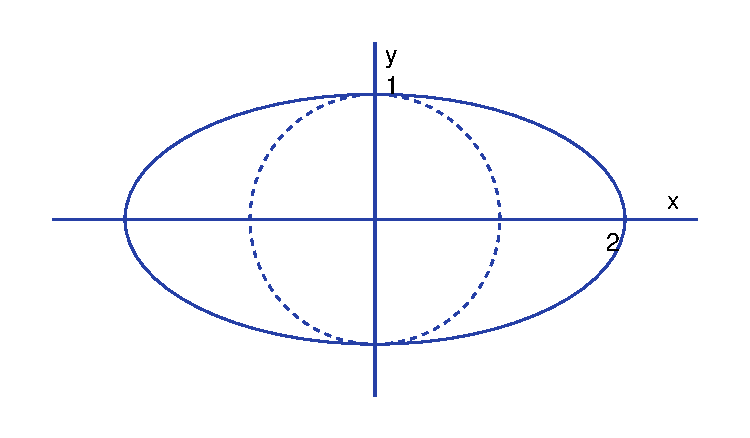
\includegraphics[width=.7\linewidth]{ellipse.pdf}
\caption{The image of the unit circle under $A=\operatorname{diag}(2,1)$.}\label{fig:ellipse}
\end{figure}
\begin{center}\begin{tabular}{ccc}\toprule
$x$ & $Ax$ & $\|Ax\|_2$\\\midrule
$(1,0)$ & $(2,0)$ & $2$\\
$(0,1)$ & $(0,1)$ & $1$\\\bottomrule
\end{tabular}\end{center}
\begin{exercise}\label{ex:diagonal}
Let $A=\operatorname{diag}(2,1)$. Find the smallest $K\geq0$ such that $\|Ax\|_2\leq K\|x\|_2$ for every $x\in\R^2$. Compare your answer with $C$ in~\eqref{eq:bound}.
\end{exercise}

\newpage
% SOURCE_PDF_PAGE: 4
\section{Review and references}
The order of quantifiers matters: one constant $C$ works for every vector $x$. The claim does not require $A$ to be invertible and does not assert that $C$ is optimal.
\begin{enumerate}
\item Identify the variables and indices in~\eqref{eq:product}.
\item Explain why taking square roots in the proof preserves the inequality.
\item Check that Figure~\ref{fig:ellipse} agrees with the table.
\end{enumerate}
For the source of this self-contained note, see~\cite{localnote}. The bibliography identifies the local source; no external mathematical citation is needed for the proof given here.
\printbibliography

\end{document}
